\chapter{Proposed solution}

% Approach
%   1. Fine-Tuning vs. Retrieval-Augmented Generation
%   2. Why BGE-M3?
%   3. Why Qwen?
%   3. Main Architecture
%     1. Local Model and Embedding System
%     2. Local Vector Store
%          1. Vector Database
%          2. Indexing (HNSW)
%     3. Query Handling and Prompt Management
%          1. Contextual Memory
%     6. VSCode Integration
%          1. Extension Interface
%          2. Execution and Resource Management
%     7. User Interface for Interactions
%          1. Code Suggestions and Explanations
%          2. Feedback Loop

\section{Fine-tuning vs. RAG}

\subsection{Fine-tuning}

Fine-tuning involves adapting a pre-trained LLM to specific tasks or domains by further training it on a targeted dataset. This process refines the model's parameters to align with specialized requirements, enhancing its performance in particular applications.

\begin{figure}[H]
    \centering
    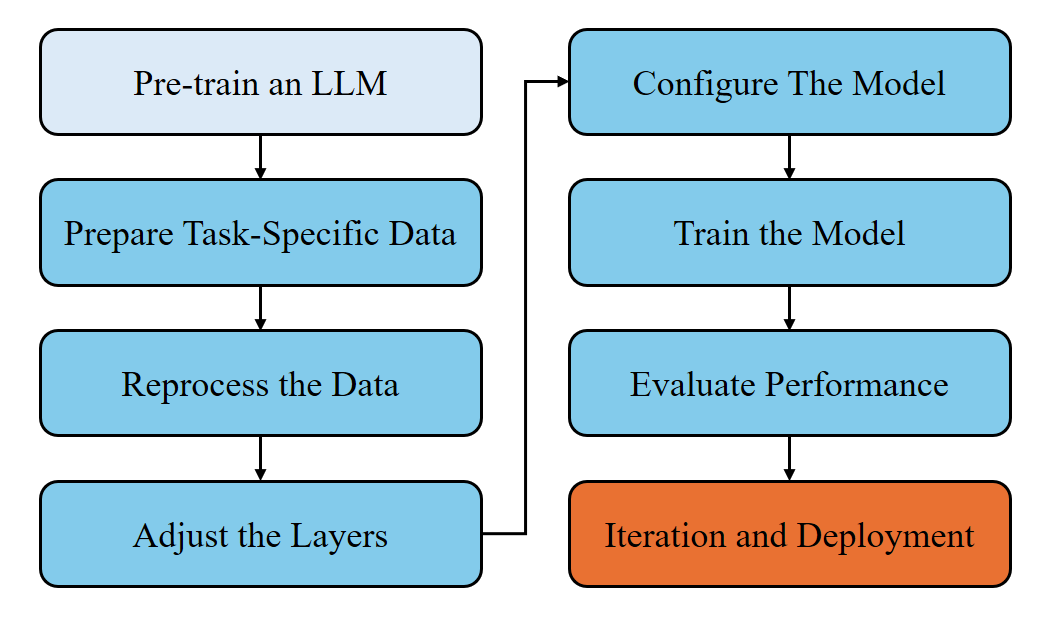
\includegraphics[width=0.7\textwidth]{Images/Approach/fine_tuning_process_diagram.png}
    
    % [Caption for LOF]{Real caption\footnotemark}
    \vspace*{4mm}
    \caption{Fine-tuning process\protect\footnotemark}
    \label{fig:fine_tuning_process}
\end{figure}

\footnotetext{RAG vs Fine-Tuning: A Comparative Analysis of LLM Learning Techniques - \url{https://addepto.com/blog/rag-vs-fine-tuning-a-comparative-analysis-of-llm-learning-techniques/}}

\subsection{Comparison between fine-tuning and RAG}

\begin{table}[H]
    \centering
    \label{tab:comparison_ft_rag}
    \begin{tabular}{p{3cm}p{6cm}p{6cm}}
        \hline
        \textbf{Aspect} & \textbf{Fine-tuning} & \textbf{RAG} \\
        \hline
        Dynamic vs. Static & Static. Relies on pre-trained knowledge, requiring retraining to update information & Dynamic. Accesses up-to-date external data sources, providing current information without retraining \\
        \hline
        Architecture & Utilizes a pre-trained LLM adjusted with task-specific datasets & Combines LLM with external knowledge bases, enabling retrieval and generation \\
        \hline
        Customization & High customization in domain-specific knowledge, tone, and style & Limited customization to domain behavior but excels in integrating external content \\
        \hline
        Hallucinations & Reduces hallucinations through domain-specific training & Minimizes hallucinations by grounding responses in retrieved documents \\
        \hline
        Accuracy & High accuracy in specific, trained domains but limited outside the training scope & Highly accurate for retrieving up-to-date, domain-relevant information \\
        \hline
        Transparency & Functions as a "black box" with limited insight into response reasoning & Transparent response generation with traceable data sources \\
        \hline
        Cost & Higher cost due to significant computational resources, and periodic retraining for updates & Lower cost as it eliminates the need for retraining by leveraging external knowledge bases \\
        \hline
        Complexity & More complex due to the need for expertise in NLP, deep learning, and hyperparameter tuning & Simpler to set up with minimal coding for retrieval integration \\
        \hline
        Adaptability & Less adaptable, requiring retraining for new information & Easily adapts to new data and dynamic environments \\
        \hline
    \end{tabular}
    \caption{Comparison of fine-tuning and RAG}
\end{table}

\begin{figure}[H]
    \centering
    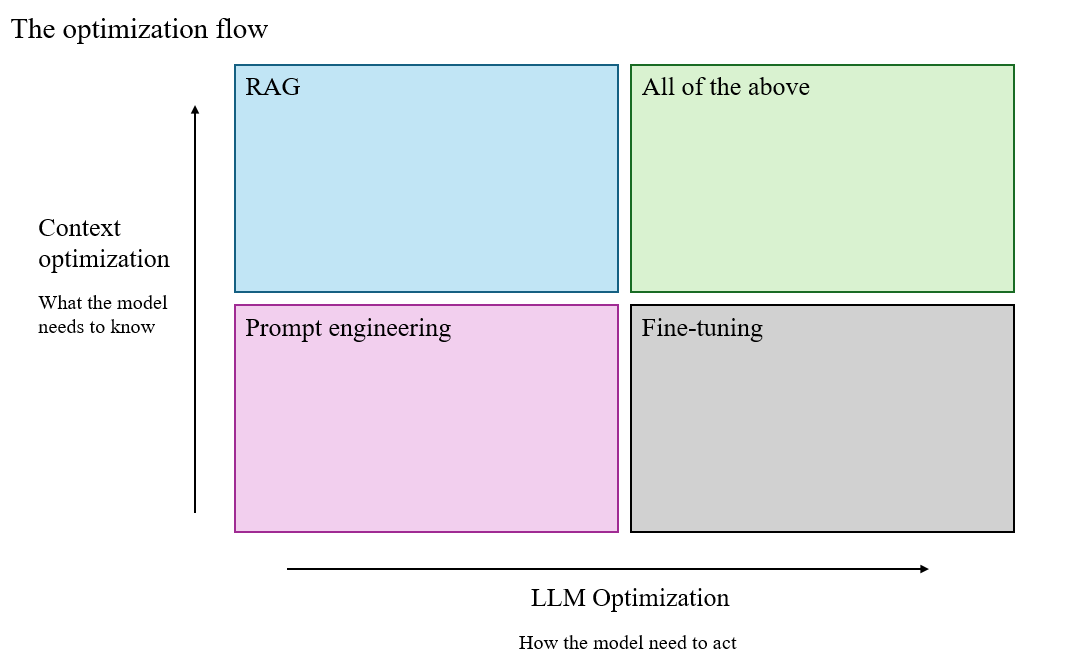
\includegraphics[width=0.7\textwidth]{Images/Approach/The nature of Fine-Tuning and RAG.png}
    
    \vspace{3mm}
    \caption{The nature of fine-tuning and RAG\protect\footnotemark}
\end{figure}

\footnotetext{Fine-tuning vs. RAG: Understanding the Difference - \url{https://finetunedb.com/blog/fine-tuning-vs-rag/}}


\subsection{Rationale for choosing RAG}

\paragraph*{Minimize hallucinations with minimal cost.} RAG provides real-time access to the latest documentation and programming guidelines, ensuring that code suggestions are current and precise without the need for extensive retraining.

\paragraph*{Transparency.} By grounding responses in specific, retrievable documents, RAG offers clear traceability of information sources. This transparency fosters trust in the generated outputs, as developers can verify the origins of the suggestions provided.

\section{Main architecture} \label{sec:main_archi}

Our system, called RAGGIN (Retrieval-Augmented Generation for Guided Intelligence in Next.js) is composed of the following key components:

\begin{itemize} 
	\item \textbf{Vector database.} Stores the Next.js documentation in an optimized vector format to enable efficient semantic retrieval. 
	\item \textbf{Retriever.} Accepts the user query sent from the VS Code extension and retrieves the most relevant documents from the vector database. 
	\item \textbf{Augmentation.} Combines the user query and retrieved documents to construct a context-rich prompt, including relevant context and additional questions, and forwards it to the generator. 
	\item \textbf{Generator.} Receives the augmented prompt and utilizes the local LLM to generate accurate and contextually relevant responses. 
\end{itemize}

\begin{figure}[H]
	\vspace{2pt}
	\centering
	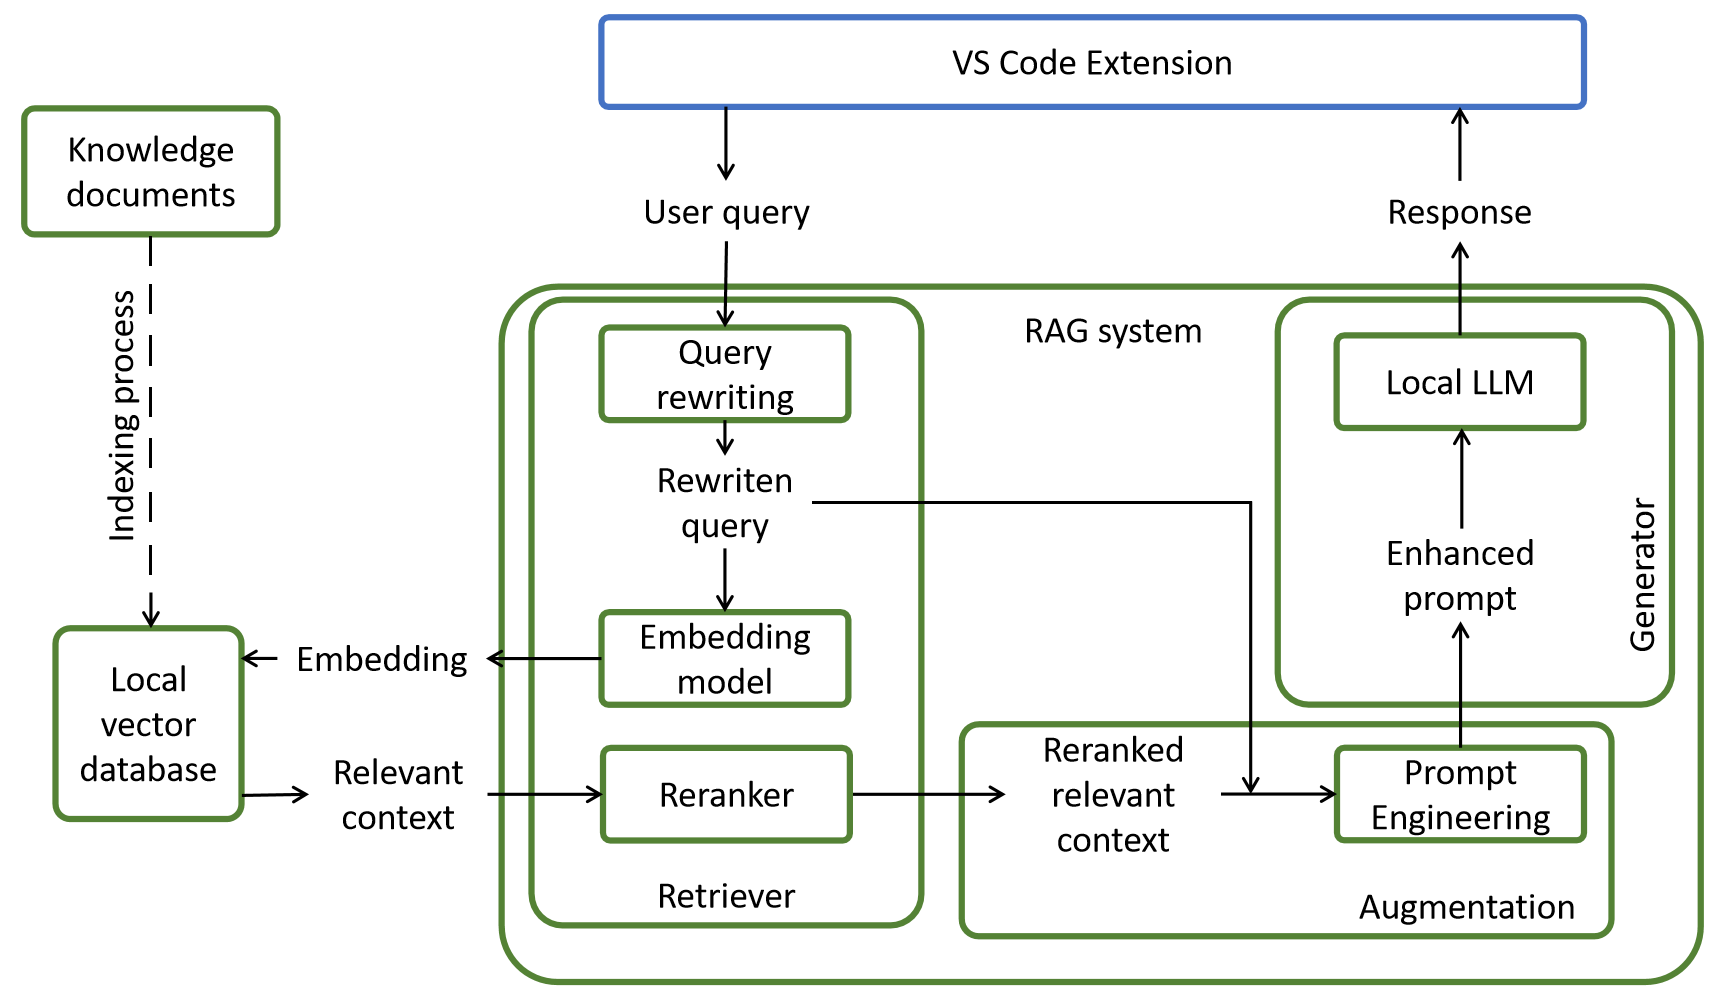
\includegraphics[scale=0.5]{Images/Implement/rag_pipeline.png}
	\vspace{5mm}
	\caption{RAGGIN architecture design}
	\label{fig:RAGGIN-architecture}
\end{figure}

The proposed RAGGIN system is designed to address the key issues outlined in Section \ref{problem_statement} by combining advanced retrieval and generation techniques with seamless integration into the developer workflow. Below is how the system resolves the identified problems.

\begin{itemize}
	\item \textbf{Disruption of workflow.} RAGGIN delivers in-editor assistance, eliminating the need for developers to leave the code editor to consult external documentation or perform browser-based searches. This minimizes context switching and preserves development focus.
	
	\item \textbf{Outdated or irrelevant context.} By retrieving documentation based on the specified version of the framework, RAGGIN ensures that the information provided is accurate and contextually aligned with the developer’s current environment, reducing the risk of relying on obsolete or generalized content.
\end{itemize}

\section{Why Milvus?}

Milvus is our chosen vector database for storing embedded data in the system. This decision is based on several compelling reasons:

\begin{itemize}
	\item \textbf{Open source.} 
	Milvus is an open-source database, perfectly aligning with our vision of delivering a free, open-source, distributed code assistance tool for VS Code. Its open nature encourages transparency and community contributions.
	
	\item \textbf{Support for structured and unstructured data.} 
	The nature of our dataset, comprising both structured metadata (e.g., documentation sections, categories) and unstructured content (e.g., textual descriptions, code snippets), makes Milvus an ideal choice. Structured data benefits from attribute-based filtering, allowing users to narrow their queries to specific documentation sections. Meanwhile, unstructured data, such as free-form text and code snippets, is embedded into high-dimensional vectors for similarity-based retrieval.
	
	\item \textbf{Comprehensive SDK and model support.} 
	Milvus's SDK seamlessly integrates with our chosen embedding model, BGE-M3, for generating high-quality embeddings. It also supports the HNSW algorithm for efficient indexing of unstructured data. This compatibility with our preferred methods ensures smooth implementation and reliable performance.
	
	\item \textbf{Scalability.} 
	Milvus employs LSM-based storage to minimize disk I/O and ensure efficient handling of frequent updates. This scalability is critical for managing dynamic and evolving datasets, such as continuously updated framework documentation.
	
	\item \textbf{Performance.} 
	Since our system is designed to run entirely on the user's local machine, Milvus's ability to leverage both CPU and GPU resources significantly enhances performance. This ensures that computationally intensive tasks, such as vector similarity searches and indexing, are executed efficiently, maintaining a responsive user experience.
\end{itemize}

\begin{table}[H]
	\hspace{-1.5cm}
	\begin{tabular}{lp{2cm}p{1.5cm}p{1cm}p{1.6cm}p{2cm}p{2cm}}
		\hline
		\textbf{System}                   & \textbf{Billion-Scale Data} & \textbf{Dynamic Data} & \textbf{GPU} & \textbf{Attribute Filtering} & \textbf{Multi-Vector Query} & \textbf{Distributed System} \\ \hline
		Facebook Faiss \cite{douze2024faiss, johnson2017similarity}      & \checkmark                  & \xmark                & \checkmark  & \xmark                     & \xmark                      & \xmark                     \\ \hline
		Microsoft SPTAG \cite{ChenW18}     & \checkmark                  & \xmark                & \checkmark  & \xmark                     & \xmark                      & \checkmark                 \\ \hline
		ElasticSearch \cite{elasticsearch} & \xmark                      & \checkmark            & \xmark      & \checkmark                 & \xmark                      & \checkmark                 \\ \hline
		Jingdong Vearch \cite{li2019visualsearch, li2019design}    & \checkmark                  & \checkmark            & \checkmark  & \checkmark                 & \xmark                      & \checkmark                 \\ \hline
		Alibaba AnalyticDB-V \cite{wei2020analyticdbv} & \checkmark              & \checkmark            & \xmark      & \xmark                     & \xmark                      & \checkmark                 \\ \hline
		Alibaba PASE (PostgreSQL) \cite{pase2020} & \xmark                  & \checkmark            & \xmark      & \checkmark                 & \xmark                      & \checkmark                 \\ \hline
		\rowcolor[HTML]{D3D3D3} 
		Milvus \cite{wang2021milvus}              & \checkmark                  & \checkmark            & \checkmark  & \checkmark                 & \checkmark                  & \checkmark                 \\ \hline
	\end{tabular}
	\caption{Vector database comparison}
\end{table}

\section{Why BGE-M3?}

In RAG systems, the quality of embeddings plays a critical role in determining the relevance and precision of retrieved content. BGE-M3 \cite{chen2024bge}, a state-of-the-art embedding model, has demonstrated superior performance in multilingual retrieval tasks, as shown in Table \ref{tab:bge_m3_comparison}. Compared to baseline models such as BM25 \cite{bm25}, mDPR \cite{mdpr}, mContriever \cite{mcontriever}, mE5\textsubscript{large} \cite{wang2024e5}, E5\textsubscript{mistral-7b} \cite{wang2024e5_improve}, BGE-M3 achieves an average retrieval score of 71.5 on the MIRACL dataset \cite{miracl}, significantly outperforming prior methods. This score reflects its advanced ability to generate robust and semantically meaningful representations.

The strength of BGE-M3 lies in its ability to unify dense retrieval, sparse retrieval, and multi-vector retrieval techniques. This integration allows it to handle diverse query types with high accuracy and flexibility. Notably, its performance exceeds that of other models in the M3-Embedding framework, with its "All" configuration achieving the highest score by combining the strengths of different retrieval approaches.

In our RAG pipeline, BGE-M3 serves as the foundation for the retrieval stage, ensuring that only the most relevant and semantically precise information is retrieved from the vector database. By leveraging BGE-M3’s advanced capabilities, we aim to enhance the overall effectiveness of the RAG system by improving the quality and relevance of the retrieved context, thus contributing to more accurate and contextually appropriate responses.

\begin{table}[h!]
	\centering
	\begin{tabular}{l c}
		\hline
		\textbf{Model}               & \textbf{Avg Score} \\ \hline
		\multicolumn{2}{l}{\textbf{Baselines}} \\ \hline
		BM25 \cite{bm25}                         & 31.9               \\
		E5\textsubscript{mistral-7b} \cite{wang2024e5_improve} & 63.4               \\
		OpenAI-3                     & 54.9               \\ \hline
		\multicolumn{2}{l}{\textbf{M3-Embedding \cite{chen2024bge}}}  \\ \hline
		Dense                        & 69.2               \\
		Sparse                       & 53.9               \\
		Multi-vector                 & 70.5               \\
		Dense+Sparse                 & 70.4               \\
		All                          & \textbf{71.5}      \\ \hline
	\end{tabular}
	\caption{Comparison of BGE-M3 embeddings with baseline models for multi-lingual retrieval performance on the MIRACL dataset \cite{chen2024bge}}
	\label{tab:bge_m3_comparison}
\end{table}

%\section{Why Qwen?}
%
%% Qwen \cite{bai2023qwen} is a relatively less recognized yet promising LLM developed by Alibaba Cloud, designed to offer robust natural language understanding and generation capabilities. While it may not be as widely publicized or frequently used as some of its contemporaries, Qwen presents unique advantages that warrant its inclusion in our comparative study. Our goal is to use RAG techniques to evaluate how effectively "weaker" LLMs like Qwen can benefit from external knowledge sources to enhance their performance compared to more advanced models. By employing RAG, we aim to demonstrate the potential of Qwen to leverage additional information and improve its generative responses and contextual understanding. This comparative analysis will provide valuable insights into the strengths and limitations of Qwen and contribute to the ongoing research on how weaker LLMs can be enhanced through advanced techniques like RAG.
%
%
%Qwen \cite{bai2023qwen} is a relatively less recognized yet promising LLM developed by Alibaba Cloud, designed to offer robust natural language understanding and generation capabilities. While its public profile may not be as prominent as some of its contemporaries, the performance metrics in Table \ref{table:qwen} demonstrate that Qwen is highly competitive in several benchmarks. For instance, the 14B parameter Qwen model achieves state-of-the-art results in tasks such as MMLU (66.3), C-Eval (72.1), and GSM8K (61.3), surpassing many well-known local models like LLaMA \cite{llama}, Llama2 \cite{llama2} and Baichuan2 \cite{baichuan2}. This highlights Qwen’s strong capability to handle diverse tasks effectively despite having fewer parameters compared to some larger models.
%
%The decision to integrate Qwen into our RAG pipeline stems from its balance of efficiency, performance, and adaptability. By leveraging RAG, we aim to showcase how even a "lighter" LLM like Qwen can achieve substantial improvements by incorporating external knowledge sources. Unlike more resource-intensive models, Qwen's relatively lightweight architecture allows for efficient local deployment, making it a practical choice for scenarios where computational resources are limited. This approach not only aligns with our objective of building a lightweight and context-aware system but also emphasizes how RAG techniques can enhance the generative responses and contextual understanding of models that might otherwise be constrained by their architecture.
%
%This comparative analysis provides valuable insights into Qwen’s strengths and limitations, illustrating its potential as an effective and efficient solution when paired with external retrieval mechanisms in RAG-based applications.
%
%
%\begin{table}[ht]
%\centering
%\begin{tabular}{l c c c c c c c c}
%\hline
%\textbf{Model}      & \textbf{Params} & \textbf{MMLU} & \textbf{C-Eval} & \textbf{GSM8K} & \textbf{MATH} & \textbf{HumanEval} & \textbf{MBPP} & \textbf{BBH} \\ 
%                    &                 & \textbf{5-shot} & \textbf{5-shot} & \textbf{8-shot} & \textbf{4-shot} & \textbf{0-shot}    & \textbf{3-shot} & \textbf{3-shot} \\ \hline
%
%Baichuan2            & 7B             & 54.7           & 56.3           & 24.6           & 5.6           & 18.3               & 24.2          & 41.6          \\
%                    & 13B            & 59.5           & 59.0           & 52.8           & 10.1          & 17.1               & 30.2          & 49.0          \\ \hline
%LLaMA              & 7B             & 35.6           & 27.3           & 11.0           & 2.9           & 12.8               & 17.7          & 33.5          \\
%                    & 13B            & 47.7           & 31.8           & 20.3           & 4.2           & 15.8               & 22.0          & 37.9          \\
%                    & 33B            & 58.7           & 37.5           & 42.3           & 7.1           & 21.7               & 30.2          & 50.0          \\
%                    & 65B            & 63.7           & 40.4           & 54.4           & 10.6          & 23.7               & 37.7          & 58.4          \\ \hline
%Llama 2              & 7B             & 46.8           & 32.5           & 16.7           & 3.3           & 12.8               & 20.8          & 38.2          \\
%                    & 13B            & 55.0           & 41.4           & 29.6           & 5.0           & 18.9               & 30.3          & 45.6          \\
%                    & 34B            & 62.6           & 42.6           & 42.2           & 6.2           & 22.6               & 33.0          & 44.1          \\
%                    & 70B            & 69.8           & 50.1           & 63.6           & 13.5          & 29.9               & 45.0          & 64.9          \\ \hline
%QWEN                & 1.8B           & 44.6           & 54.7           & 21.2           & 5.6           & 17.1               & 14.8          & 28.2          \\
%                    & 7B             & 58.2           & 63.5           & 51.7           & 11.6          & 29.9               & 31.6          & 45.0          \\
%                    & 14B            & 66.3           & 72.1           & 61.3           & 24.8          & 32.3               & 40.8          & 53.4          \\ \hline
%\end{tabular}
%\caption{Performance comparison of some open-source base models on different benchmarks \cite{bai2023qwen}}
%\label{table:qwen}
%\end{table}
%
%\begin{table}[ht]
%	\centering
%	\begin{tabular}{l c c c c}
%		\hline
%		\textbf{Model}      & \textbf{Params} & \textbf{HumanEval} & \textbf{MATH} & \textbf{GSM8K} \\ 
%		&                 & \textbf{0-shot}    & \textbf{4-shot} & \textbf{8-shot} \\ \hline
%		Baichuan 2 \cite{baichuan2}           & 7B             & 18.3               & 5.6           & 24.6           \\ \hline
%		LLaMA \cite{llama}               & 7B             & 12.8               & 2.9           & 11.0           \\ \hline
%		Llama 2 \cite{llama2}           & 7B             & 12.8               & 3.3           & 16.7           \\ \hline
%		QWEN \cite{bai2023qwen}               & 1.8B           & 17.1               & 5.6           & 21.2           \\
%		\hline
%	\end{tabular}
%	\caption{Performance comparison of Qwen 1.8B and other 7B models on selected benchmarks}
%	\label{table:qwen_filtered}
%\end{table}

%\section{Why Ollama?}
%
%In designing a fully local RAG system, Ollama\footnote{Ollama - \url{https://ollama.com/}} was selected as the LLM runtime for its ease of use, lightweight architecture, and compatibility with a wide range of open-source models. Ollama provides a simple yet powerful API interface for serving large language models directly on local machines, removing the dependency on cloud-based inference and ensuring full control over data privacy and latency. Its support for models such as Qwen \cite{bai2023qwen}, LLaMA \cite{llama}, and Mistral \cite{mistral} makes it a versatile backend for experimentation and deployment. Moreover, the CLI-based installation and Docker integration simplify the setup process, aligning with the goal of being developer-friendly and easy to deploy. By utilizing Ollama, our system guarantees that all generation processes remain offline, making it suitable for privacy-conscious environments and offline development workflows.

\section{Why Ollama?}

In designing a fully local RAG system, Ollama\footnote{Ollama - \url{https://ollama.com/}} was selected as the LLM runtime for its ease of use, lightweight architecture, and compatibility with a wide range of open-source models. Ollama provides a simple yet powerful API interface for serving large language models directly on local machines, removing the dependency on cloud-based inference and ensuring full control over data privacy and latency. Its support for models such as Qwen \cite{bai2023qwen}, LLaMA \cite{llama}, and Mistral \cite{mistral} makes it a versatile backend for experimentation and deployment. Moreover, the CLI-based installation and Docker integration simplify the setup process, aligning with the goal of being developer-friendly and easy to deploy. By utilizing Ollama, our system guarantees that all generation processes remain offline, making it suitable for privacy-conscious environments and offline development workflows.

\vspace{0.5em}
\paragraph*{Model support and flexibility.} Ollama offers a broad library of pre-integrated models, ranging from lightweight options to very large models. Notable supported models include:
\begin{itemize}
	\item \textbf{SmolLM\footnote{SmolLM -  \url{https://ollama.com/library/smollm}}.} Models with 135M, 360M, and 1.7B parameters, optimized for resource-constrained environments.
	\item \textbf{TinyLlama\footnote{TinyLlama -  \url{https://ollama.com/library/tinyllama}}.} A compact 1.1B parameter model designed for efficiency.
	\item \textbf{DeepSeek-R1\footnote{DeepSeek-R1 - \url{https://ollama.com/library/deepseek-r1}}.} Scalable up to 671B parameters, demonstrating Ollama’s capacity to handle massive models.
	\item \textbf{LLaMA 3.1\footnote{LLaMA 3.1 - \url{https://ollama.com/library/llama3.1}}.} Supports 8B, 70B, and 405B variants, enabling flexible usage for tasks of varying complexity.
\end{itemize}

\vspace{0.5em}
\paragraph*{System compatibility.} According to the official documentation\footnote{Ollama Documentation - \url{https://github.com/ollama/ollama/tree/main/docs}}, Ollama runs on all major operating systems, including Linux, macOS, and Windows (with native support, removing the need for WSL). Recommended system requirements include:
\begin{itemize}
	\item \textbf{RAM.} 8GB for 3B models, 16GB for 7B models, and 32GB for 13B models.
	\item \textbf{CPU.} At least 4 cores (8 cores recommended for larger models).
	\item \textbf{Disk Space.} A minimum of 12GB for base installation, plus additional storage for model data.
	\item \textbf{GPU (optional).} GPU acceleration significantly improves performance and compatible with both NVDIA and AMD cards.
\end{itemize}

\vspace{0.5em}
\paragraph*{Developer ecosystem and community.} Ollama is under active development, with strong community support reflected by its large GitHub presence\footnote{Ollama Github - \url{https://github.com/ollama/ollama}}. The platform provides a Python SDK that offers an intuitive, flexible interface ideal for integrating LLMs into applications such as RAG systems. Its growing adoption, combined with simplicity and performance focus, makes it a compelling choice for local model deployment.

\section{Why Docker?}

Docker was chosen as the containerization solution for our RAG system to ensure portability, consistency, and ease of deployment across various development environments. According to Docker’s 2024 report\footnote{Docker Unveils 2024 State of Application Development Report - \url{https://www.docker.com/press-release/unveils-2024-state-of-application-development-report/}}, over 36\% of developers now use remote development environments such as GitHub Codespaces, Gitpod, and Coder, indicating a strong shift away from traditional local development toward cloud-based workflows. This trend reinforces the importance of containerization in providing a consistent, reproducible environment for development and deployment.
		
Our backend comprising retrieval services, embedding logic, and vector database integration is relatively complex and contains multiple dependencies that are difficult to configure manually. Docker allows us to encapsulate these components into isolated containers, enabling users to launch the full backend stack with a single command, regardless of operating system or local setup.
		
Additionally, the report shows that 64\% of developers have integrated AI tools into their development workflows, especially for coding, documentation, and research. Docker helps simplify the deployment of AI/ML components and ensures they can be reused consistently across teams. By abstracting away the configuration complexity of tools like the Milvus vector database and embedding models, Docker facilitates smoother onboarding, maintenance, and scalability.
		
Finally, Docker’s support for volume mounting and environment variables offers flexibility in managing different versions of models, data, and configurations, without altering the core codebase, making it an ideal solution for modern AI-powered systems like ours.

\section{Why VS Code extension?}

Integrating the RAG system into a VS Code extension offers a seamless and efficient experience for developers by embedding AI-powered support directly into their primary development environment. This approach minimizes context-switching and enhances productivity by allowing developers to query documentation, generate code, and receive intelligent suggestions in real time, without leaving the editor.
 
The interactive user interface of the VS Code extension is designed to optimize the developer's workflow. By eliminating the need to switch between the code editor and external resources like browsers or documentation portals, the system reduces distractions and streamlines the development process. Integration into the editor also allows direct access to the active codebase, enabling context-aware recommendations and code generation tailored to the current task.

%VS Code is the most widely adopted Integrated Development Environment (IDE) among web developers\footnote{2024 Stack Overflow Developer Survey - \url{https://survey.stackoverflow.co/2024/technology\#most-popular-technologies-new-collab-tools}}. Its robust support for terminals, extensions, and custom interfaces makes it an ideal platform for deploying AI-assisted tools.

According to the 2024 Stack Overflow Developer Survey\protect\footnotemark, 73.6\% of developers reported using VS Code more than double the share of its nearest competitor. This wide adoption reflects the editor’s reliability, ease of use, and active community support.

\begin{figure}[H]
	\vspace{2pt}
	\centering
	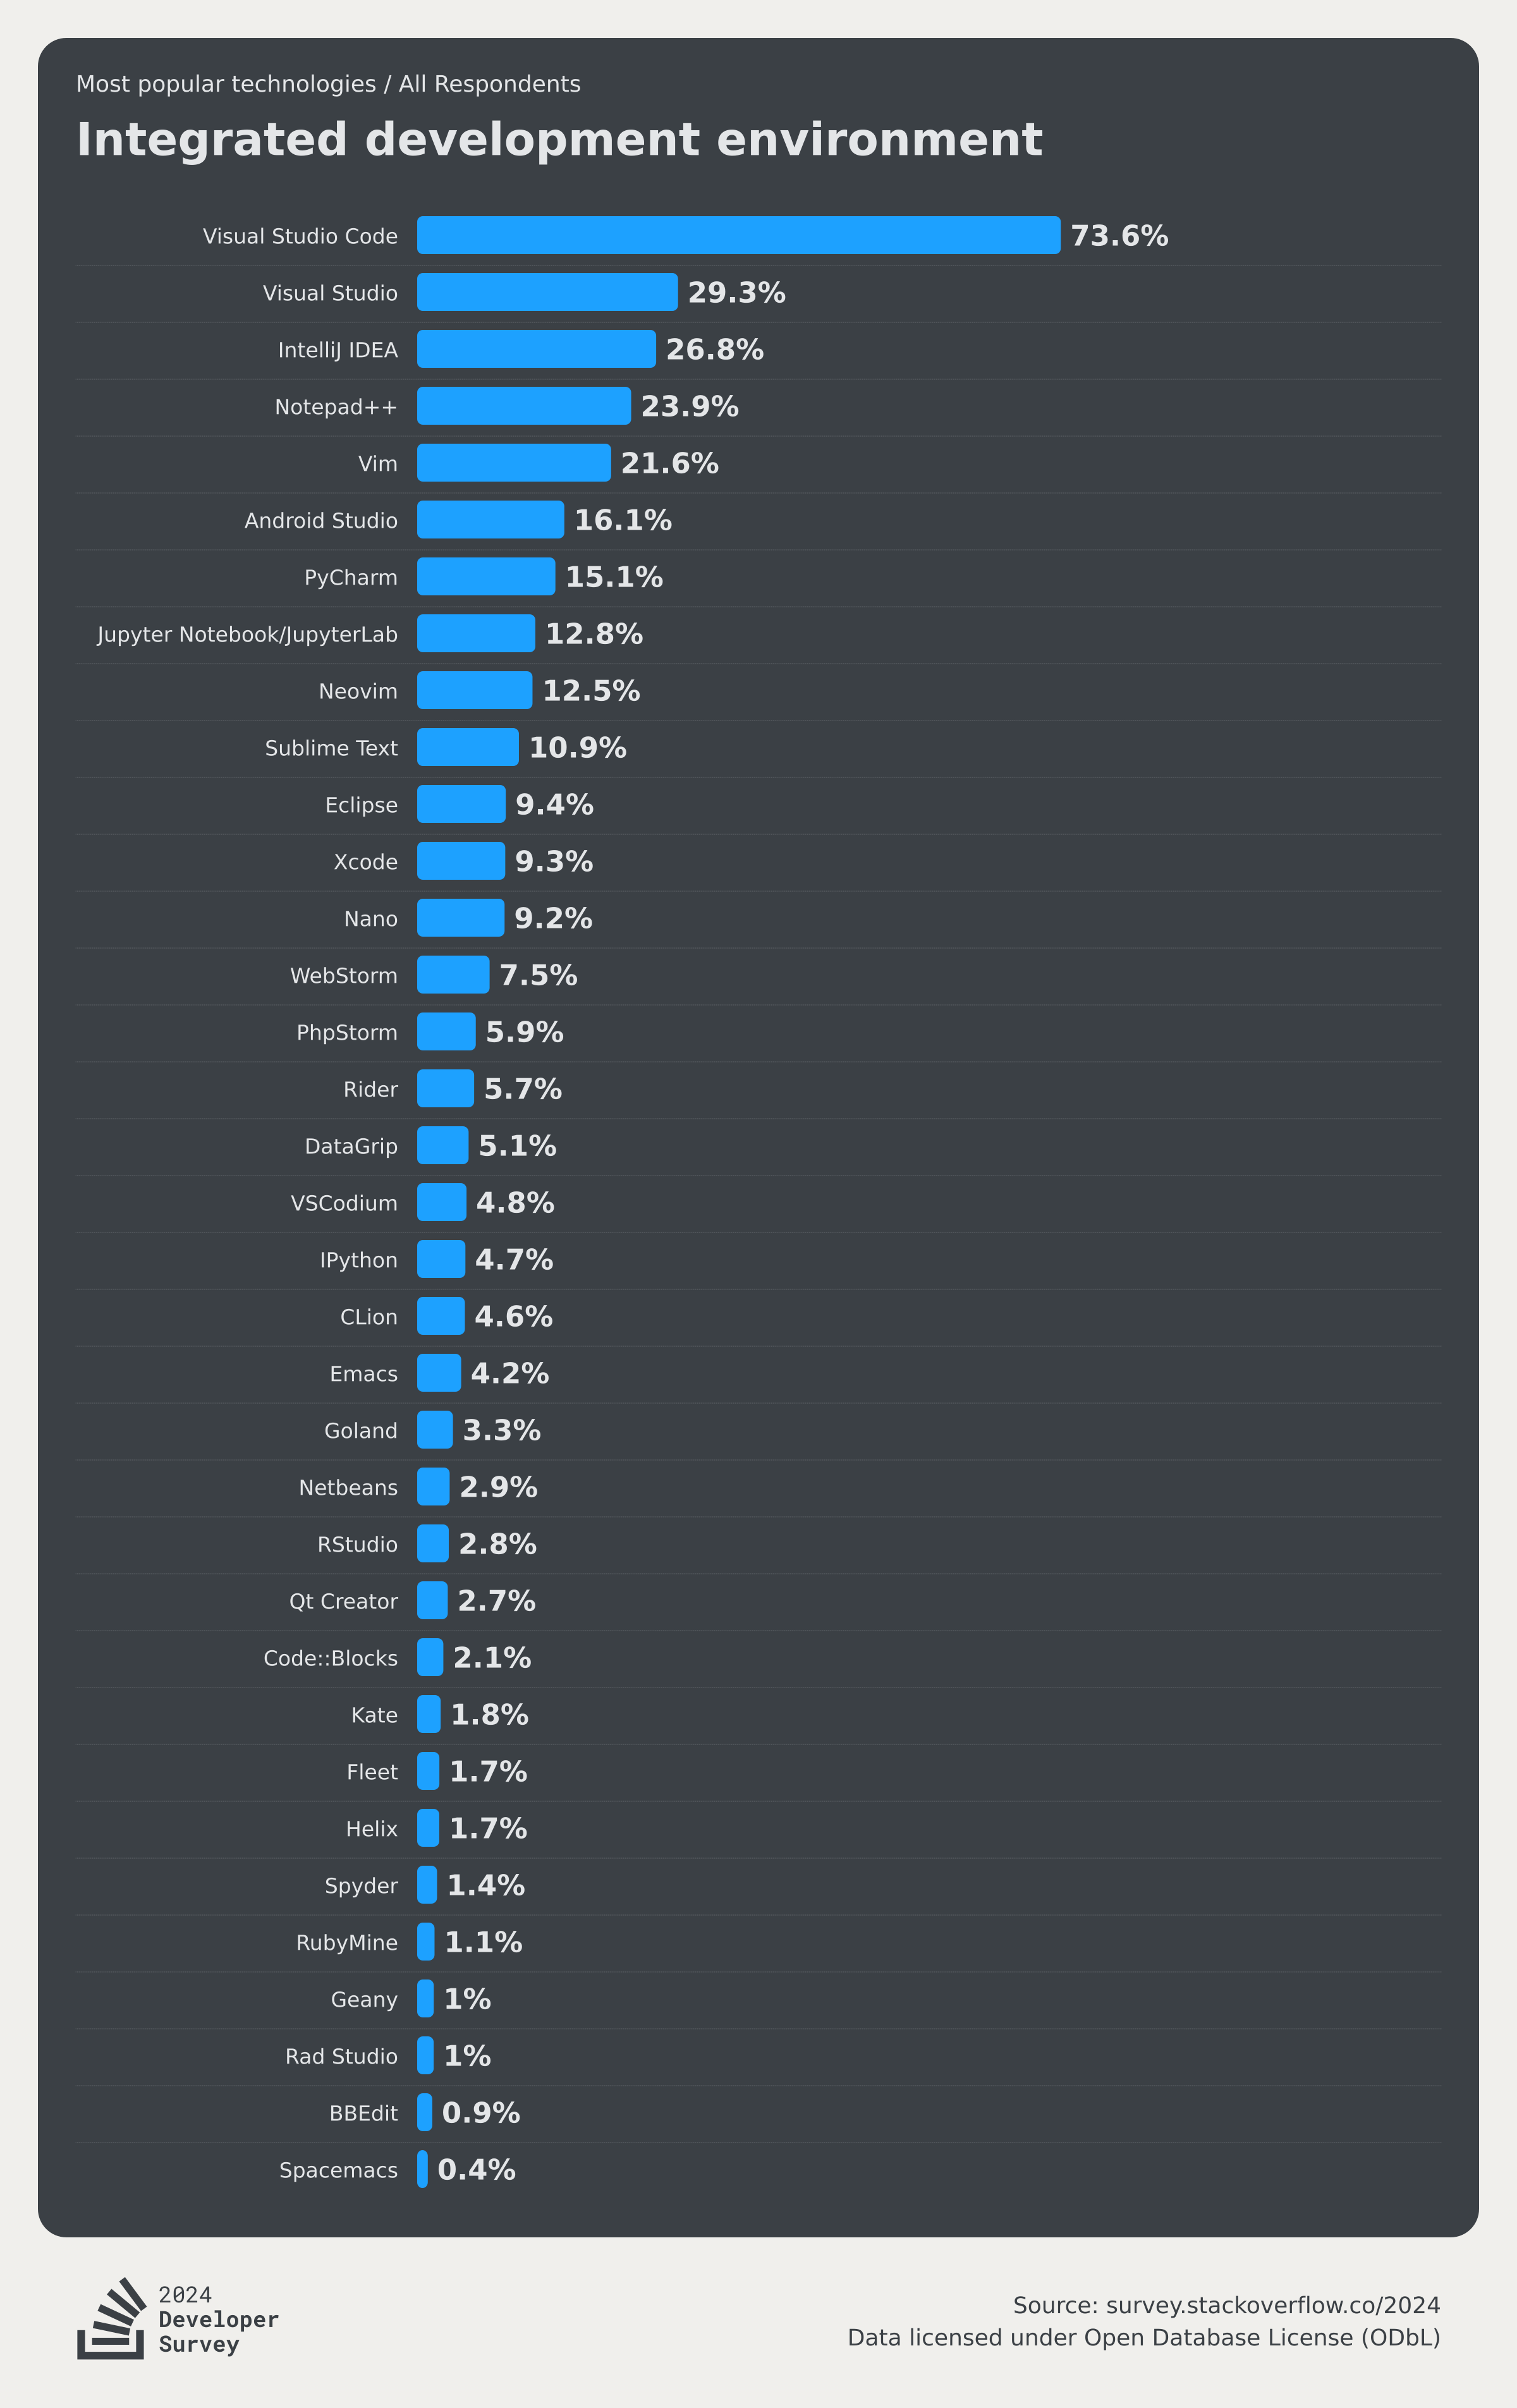
\includegraphics[width=0.8\textwidth]{Images/Approach/stackoverflow-dev-survey-2024-technology.png}
	\vspace{5mm}
	\caption{Most popular IDEs in 2024 according to the Stack Overflow Developer\protect\footnotemark.}
	\label{fig:vscode_survey}
\end{figure}

\footnotetext{2024 Stack Overflow Developer Survey - \url{https://survey.stackoverflow.co/2024/technology\#most-popular-technologies-new-collab-tools}}
